\documentclass[tikz,border=2pt]{standalone}
\usepackage{amsmath,amssymb}
\usepackage{tikz}
\usetikzlibrary{arrows.meta}

\begin{document}
% M is an upper bound of S when every element of S lies at or to the left of M; a set has many
% upper bounds (everything to the right of one is another), and the least of them is the supremum.
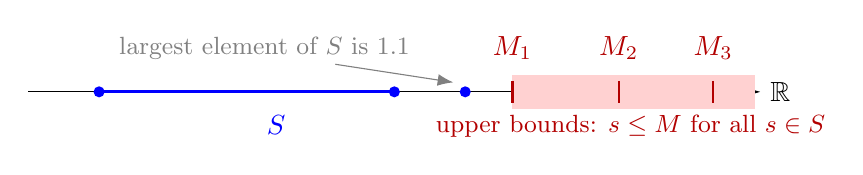
\begin{tikzpicture}[x=1.5cm]
	\draw[-{Latex[length=2.5mm]}] (-2.6,0) -- (3.6,0) node[right] {$\mathbb{R}$};
	\fill[red!18] (1.5,-0.22) rectangle (3.55,0.22);
	\draw[very thick, blue] (-2,0) -- (0.5,0);
	\fill[blue] (-2,0) circle (2pt);
	\fill[blue] (0.5,0) circle (2pt);
	\fill[blue] (1.1,0) circle (2pt);
	\node[blue, below=5pt] at (-0.5,0) {$S$};
	\foreach \x/\l in {1.5/$M_1$, 2.4/$M_2$, 3.2/$M_3$} {\draw[red!70!black, thick] (\x,0.14) -- (\x,-0.14); \node[red!70!black, above=4pt] at (\x,0.14) {\l};}
	\node[red!70!black, below=5pt, font=\small] at (2.5,0) {upper bounds: $s\le M$ for all $s\in S$};
	\node[gray, above=4pt, font=\small] at (-0.6,0.15) {largest element of $S$ is $1.1$};
	\draw[-{Latex[length=2mm]}, gray] (0.0,0.35) -- (1.0,0.12);
\end{tikzpicture}
\end{document}
